%arara : pdflatex
\documentclass[12pt]{article}

\usepackage{../style/style}

\begin{document}

\def\reporttitle{Réalisation d'un mini-compilateur pour le langage: TinyLanguage\_SII en utilisant ANTLR avec génération du code objet.}
%----------------------------------------------------------------------------------------
%	TITLE PAGE
%----------------------------------------------------------------------------------------


\begin{titlepage} % Suppresses displaying the page number on the title page and the subsequent page counts as page 1
	\newcommand{\HRule}{\rule{\linewidth}{0.5mm}} % Defines a new command for horizontal lines, change thickness here
	
	\center % Centre everything on the page
	
	%------------------------------------------------
	%	Headings
	%------------------------------------------------
	
	\baselineskip=2\baselineskip 
	\textsc{\LARGE Université des Sciences et de la Technologie Houari Boumediene}%\\[1cm] % Main heading such as the name of your university/college

	%------------------------------------------------
	%	Logo
	%------------------------------------------------
	
	%\vfill\vfill
	\vfill
	
\includegraphics[width=0.3\textwidth]{../../TP0/USTHB_Logo.png}\\[1cm] % Include a department/university logo - this will require the graphicx package
	 
	%----------------------------------------------------------------------------------------
	
	\textsc{\Large Conception et Complexité des Algorithme}\\[0.5cm] % Major heading such as course name
	%\textsc{\large Minor Heading}\\[0.5cm] % Minor heading such as course title
	
	%------------------------------------------------
	%	Title
	%------------------------------------------------
	
	\HRule\\[0.4cm]
	\baselineskip=1.2\baselineskip 
	{\huge\bfseries Rapport de Travaux Pratiques N\textdegree  \reportnumber \\ \reporttitle}\\[0.4cm] % Title of your document
	
	\HRule\\[1.5cm]
	
	%------------------------------------------------
	%	Author(s)
	%------------------------------------------------
	
	\begin{minipage}{0.4\textwidth}
		\begin{flushleft}
			\large
			\textit{Binôme}\\
			MOHAMMEDI \textsc{Haroune } % Your name
			\\
			HOUACINE  \textsc{Naila Aziza} % Your name
		\end{flushleft}
	\end{minipage}
	~
	\begin{minipage}{0.4\textwidth}
		\begin{flushright}
			\large
			\textit{Professeur}\\
			Pr. AMANI \textsc{Ferhat} % Supervisor's name
		\end{flushright}
	\end{minipage}
	
	%------------------------------------------------
	%	Date
	%------------------------------------------------
	
	\vfill\vfill\vfill % Position the date 3/4 down the remaining page
	
	{\large\today} % Date, change the \today to a set date if you want to be precise
	
	
	\vfill % Push the date up 1/4 of the remaining page
	
\end{titlepage}


\tableofcontents
\setcounter{tocdepth}{3}

\newpage


\section{Section obligatoire.}
\subsection{Étapes d'installation d'ANTLR }

Etapes d'installation d'ANTLR sous Linux (UBUNTU)\\

La procédure d'installation peut se résumer dans ces trois étapes : \\
\begin{enumerate}
    \item \textbf{Première étape:} télécharger le fichier \texttt{.jar} de l'outil.
    \item \textbf{Deuxième étape:} mettre le fichier dans le \texttt{CLASSPATH} pour que java puisse le trouver. 
    \item \textbf{Troisième étape:} création d'un alias pour le programme de tel sorte que l'on puisse l'appeler facilement.(optionnel)
\end{enumerate}

\subsubsection{Commandes utilisées}
Ainsi nous avons exécuter les commandes suivantes dans un terminal  bash:\\
\texttt{ }\\
Se positionner dans le bon répertoire.
\begin{sql}
cd /usr/local/lib
\end{sql}
\texttt{ }\\
Télécharger ANTLR du lien donné.
\begin{sql}  
sudo curl -O http://www.antlr.org/download/antlr-4.7-complete.jar
\end{sql}
\texttt{ }\\
Exporter le fichier .jar d'ANTLR dans le classpath.
\begin{sql}
export CLASSPATH=".:/usr/local/lib/antlr-4.0-complete.jar:\\char36CLASSPATH"
\end{sql}
\texttt{ }\\
Créer un alias antlr4
\textbf{}
\begin{sql}
alias antlr4="java -jar /usr/local/lib/antlr-4.0-complete.jar"
\end{sql}

\subsubsection{Problème rencontré}
Une fois le terminal fermé toutes les configurations faites précédemment sont oubliées, donc elle ne reste que le temps d'ouverture du terminale.\\

\subsubsection{Solution aux problèmes}
Rendre les configurations globales en exécutant les commandes suivantes:\\
- Ajouter la commande 
\begin{sql} 
export 
\end{sql} 
Dans le fichier \textbf{.bash\_profile} et la commande 
\begin{sql}
alias
\end{sql}
Dans le fichier \textbf{.bashrc}, ces deux derniers fichiers se trouve dans le dossier \textbf{HOME}. \\

Et enfin l'exécution des commandes : 
\begin{sql} 
bash .bash\_profile 
bash .bashrc
\end{sql} 
pour exécuter les fichiers précédents.


 

\subsection{Présentation des Différentes Phases de notre Compilateur}
\subsubsection{Analyse Lexicale}
Lors de cette étape nous avons étudié le langage du mini compilateur de l'énoncé,\\
Puis défini les entités lexicales, tel que :
-	Int, float, string, comment, progname, les identifiants  …\\

Sachant qu'on doit d'abord définir l'expression régulière du PROGNAME (nom du programme) avant la définition ID (identifiants des variables)
pour que le nom du programme ne doit pas considéré comme un identifiant d'une variable et ne pas l'insérer dans la Table des Symboles plus tard dans l'analyse sémantique.\\

L'on peut noter que pour la définition du format de l'expression d'un FLOAT nous avons réutiliser la définition du format d'un INT.\\

Puis nous avons définit l'expression régulière d'un commentaire sur plusieurs lignes ainsi que le text acceptable pour les printcompil.\\

\begin{sql}

PROGNAME : [A-Z]+[a-zA-Z0-9_]* ;
ID : [a-zA-Z]+[a-zA-Z0-9]* ;

INT :   '0' | [1-9] [0-9]* ; // no leading zeros

FLOAT
    :   '-'? INT '.' INT
    |   '-'? INT
    ;


COMMENT : '/*' .*? '*/' -> channel(HIDDEN) ;

TEXT : '"' (~'"'|'\\"')* '"'  ;

WS : [ \t\n\r]+ -> channel(HIDDEN) ;

\end{sql}
\textbf{ }\\
Pour finir nous avons enregistré se fichier sous le format \textbf{.g4} afin qu'il soit traitable (lisible) par le parser d'ANTLR.\\

\textbf{ }\\
\subsubsection{Analyse Syntaxique}
Toujours dans le même fichier \textbf{.g4}, nous avons définit la structure générale d'un programme acceptable par notre langage, qui se présente comme suit :
\begin{sql}
start_rule : 'compil' PROGNAME '(' ')'
'{'
declarations
'start'
instructions
'}';
\end{sql}

Puis chaque nonTérminale est détaillé en respectant les règles LL(k) ainsi que les spécifications de l'énoncé. \\
ci-dessous un exemple, l'instruction d'affectation :
\begin{sql}
instAff:    identifier '=' expression;
\end{sql}
Avec : \\
\textbf{instAff:} la règle de définition d'une instruction d'affectation.\\
\textbf{identifier:} La règle qui définit un identifiant ID, comme suit:
\begin{sql}
identifier : ID ;
\end{sql}
\texttt{ }\\
\textbf{expression:} la règle de définition de la composition d'une expression.\\
Elle est composée d'une succession de valeurs, identifiants et opérations arithmétiques, et prend en considération la priorité des opérateurs et leur ordre d'apparition.
\begin{sql}
expression : expression pm expression1 | expression1;
expression1 : expression1 md expression2 | expression2;
expression2 : identifier | '(' expression ')' | value ;
\end{sql}
\texttt{ }\\
Avec la définition suivante des règles pm et md:\\
(ici : pm représente la première lettre des deux mots "Plus" "+" et "Moins" "-"\\
et : md représente la première lettre des deux mots "Multiplication" "*" et "Division" "/" ).

\begin{sql} 
pm : (PLUS|MINUS) ;
md : (MULT|DIV) ;
\end{sql}
\texttt{ }\\

Et ainsi de suite pour toutes les instructions demandées (IF, SCANcompil, PRINTcompil, Affectation, les opérations sur les expressions) mais aussi d'autres instructions supplémentaires tel que FOR, WHILE, SWITCH…CASE, ... \\

En plus de cela pour chaque Terminal devant déclencher une action lors de sa rencontre par le parser, doit être définit comme règle unaire (qui génère un seul Terminale ou mot clé de notre langage).\\
puis remplacer toutes ses utilisation (référence) par la nouvelle règle le générant; si-dessous quelques exemple:\\

\begin{sql}
FOR : 'for';
WHILE : 'while';
PLUS : '+';
MINUS : '-';
MULT : '*';
DIV : '/';
...
..
.
\end{sql}


\subsubsection{Analyse Sémantique}
Lors de cette phase, nous avons donné une sémantique à nos entité, et vérifié la cohérence de notre programme à travers des routines (avec insertion dans la Table des symboles) , \\
Aussi nous avons généré la forme intermédiaire correspondante au langage développé sous forme de Quadruplets.\\

Dans ce qui suit nous allons détailler les classes crées à cet effet:\\
\texttt{ }\\ 
 
\color{blue}
-	Table des symboles : \\
\color{black}
Notre table des symboles (dans la classe « TabSymbole ») est une ArrayList de ligne, tel que chaque ligne est composée de trois (3) informations qui sont :\\
\texttt{ }\\
•	Name : l'identifiant de la variable \\
•	Type : le type de la variable\\
(qui peut être soit un « int » représenté par la valeur 1,\\
 soit un « float » représenté par la valeur 2)\\
•	Declared : booleen permettant de vérifier si une variable utilisé dans le code a été déclaré au préalable.\\

Aussi nous avons les méthodes de manipulation des éléments de la Table des Symboles :\\
\texttt{ }\\
•	getLigne : pour récupérer une ligne à partir du nom d'une variable.\\
•	containsLigne : pour tester si une variable existe dans la TS\\
•	addLigne : pour insérer une nouvelle ligne à la Table des Symboles.\\
•	getSize : pour connaitre le nombre de ligne dans la TS\\
•	toString et display : pour afficher l'intégralité de la Table des Symboles\\

\color{blue}
-	Routines :\\
\color{black}
Dans la classe « RoutinesTabSymbol » que nous avons fait hériter du « baseListner » nous avons pour chaque événement « enter » ou « exit » d'une règle implémenté les testes (routines) nécessaires, nous pouvons citer :\\
\texttt{ }\\
•	Empêcher les doubles déclarations.\\
En vérifiant le contenu de la table des symboles, si l'identifiant y est inséré, on vérifie s'il à été déclaré (champs DECLARED), sinon on génère une erreur, que l'on insert dans notre table errors.\\ 
•	Tester la compatibilité des opérandes lors des affectations, calcule des expressions ou comparaisons.\\
Pour cela nous avons utilisé un HashMap dans le quel nous avons sauvegardé le contexte comme clé puis le type de variable ou expression comme valeur, afin de tester la compatibilité avec le reste des éléments interagissant avec cette variable.\\
•	Empêcher l'utilisation de variables non déclarées.\\
A travers la recherche dans la table des symboles à chaque utilisation d'une variable.\\

Mais aussi géré l'insertion des variables dans la TS lors des déclarations, \\


\color{blue}
-	Intellij IDE :\\
\color{black}
-	Étapes de configuration d'ANTLR dans intellij\\
\textbf{ }\\
Pour l'utilisation d'ANTLR dans l'IDE Intellij, nous devons télécharger et installer le plugin \texttt{ANTLR v4 grammar plugin}, qui est accessible via l'interface d'Intellij dans:\\
File $>$ Settings $>$ Plugins $>$ puis faire une recherche d'ANTLR dans le champs de recherche visible. 
\textbf{ }\\
%image Configuration1
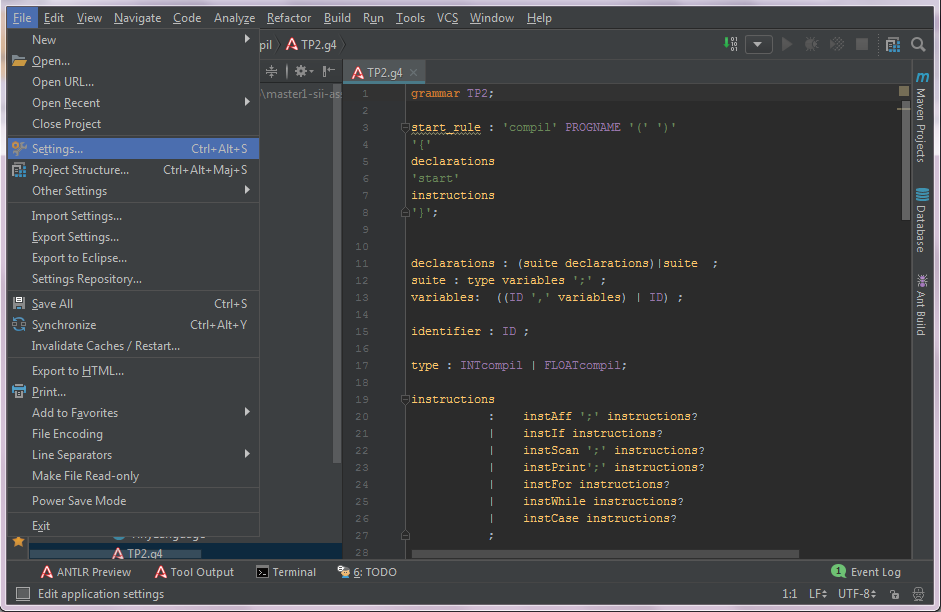
\includegraphics[width=1\textwidth]{IMG/Configuration1.png}
\textbf{ }\\
Ainsi nous sera proposé se plugin , il nous a suffit de cliquer sur installer et d'attendre quelques seconds le temps du téléchargement et installation.\\
\texttt{ }\\
%image Configuration2
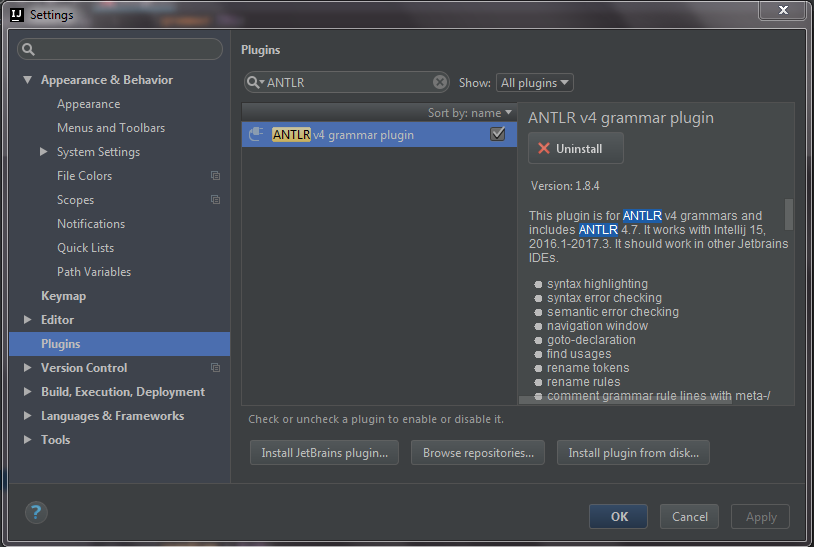
\includegraphics[width=1\textwidth]{IMG/Configuration2.png}


\texttt{ }\\
-	Génération des parser et listner\\
Pour cela il nous a suffit de faire un clique droit sur notre fichier .g4 puis de sélectionner l'option : \texttt{ Generate ANTLR recongnizer},\\
se qui engendre la création le quatre (4) classes : \\
BaseListner , BaseVisitor , Lexer et Parser \\
 en plus des Interface et fichiers tokens ...\\
\texttt{ }\\
%image Generer
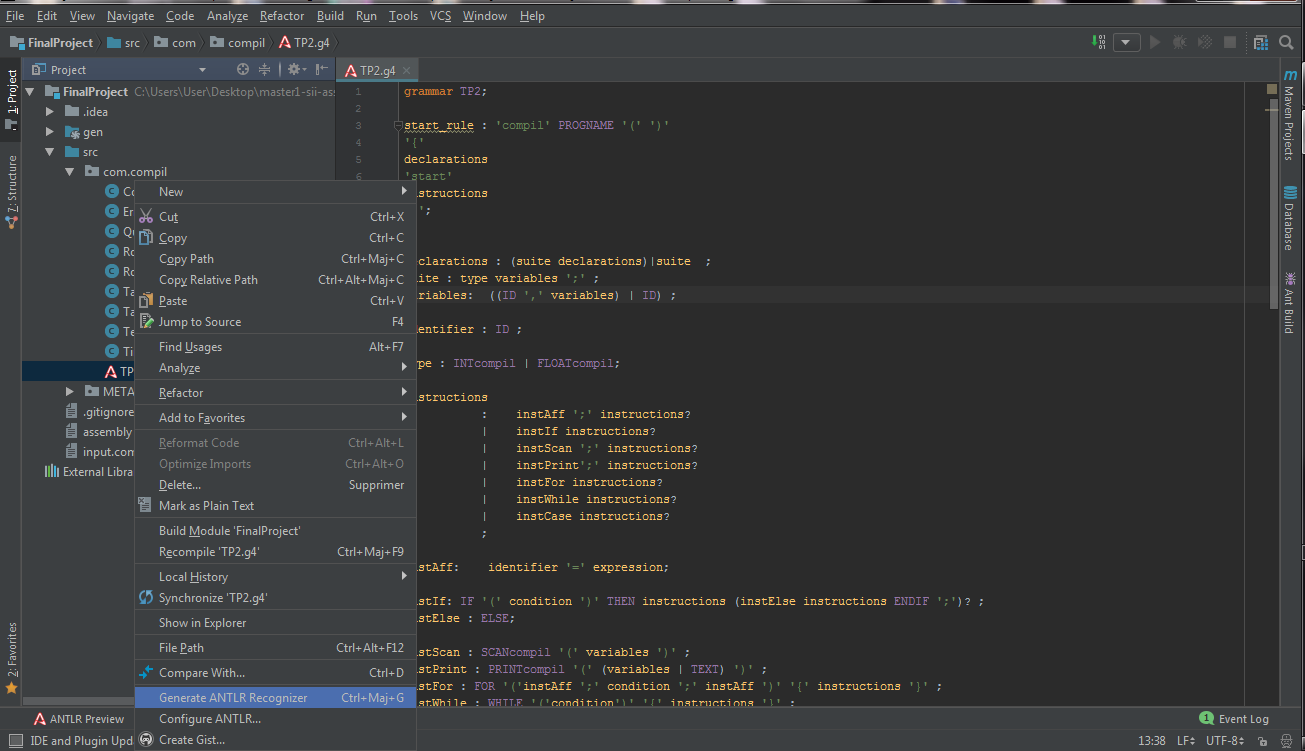
\includegraphics[width=1\textwidth]{IMG/Generer.png}


\texttt{ }\\
-	Tester les règles (arbre)\\
\texttt{ }\\
Afin de générer l'arbre syntaxique et de tester nos règles produite lors de l'analyse syntaxique, nous devons faire un clique droit sur la règle à tester puis sélectionner l'option : \texttt{Test rule start\_rule} comme suit:\\
\texttt{ }\\
%image TestRule
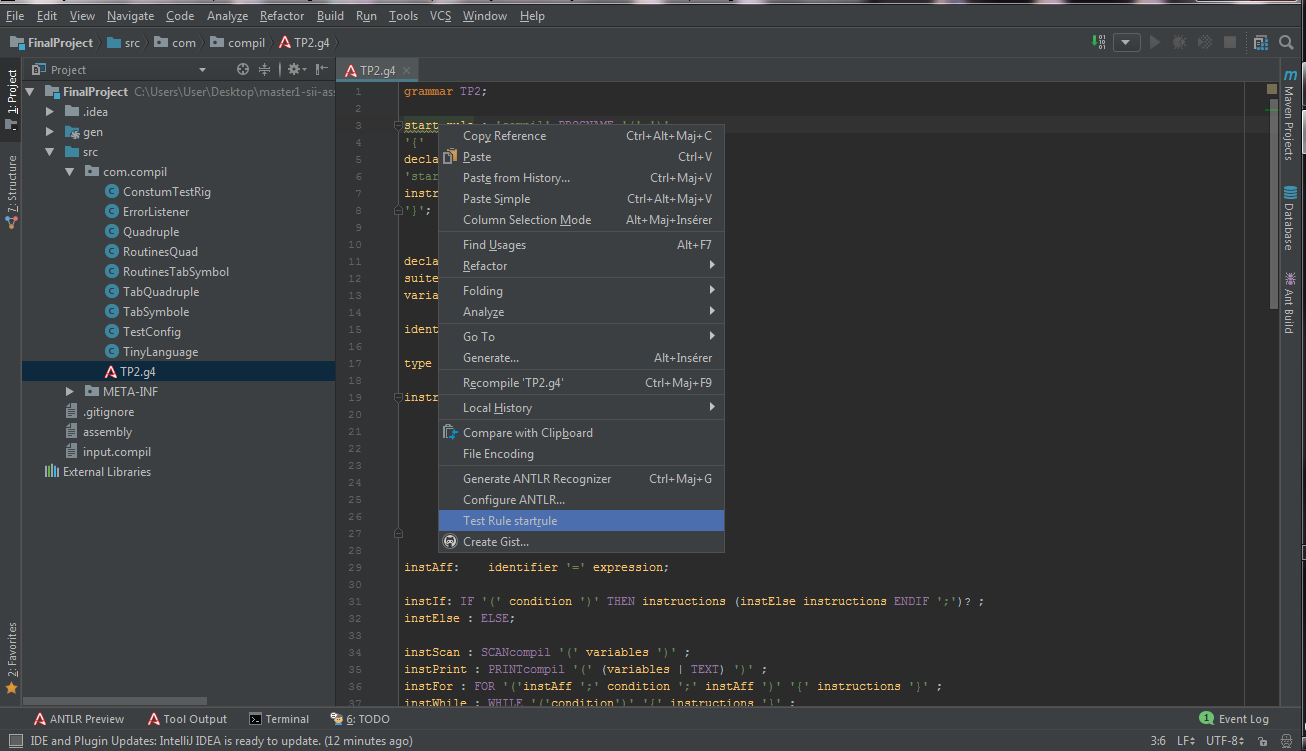
\includegraphics[width=1\textwidth]{IMG/TestRule.png}
\texttt{ }\\
Ainsi si aucun conflit n'a été détecté l'arbre sera affiché comme ci-dessous:\\
\texttt{ }\\
%image TestRule2
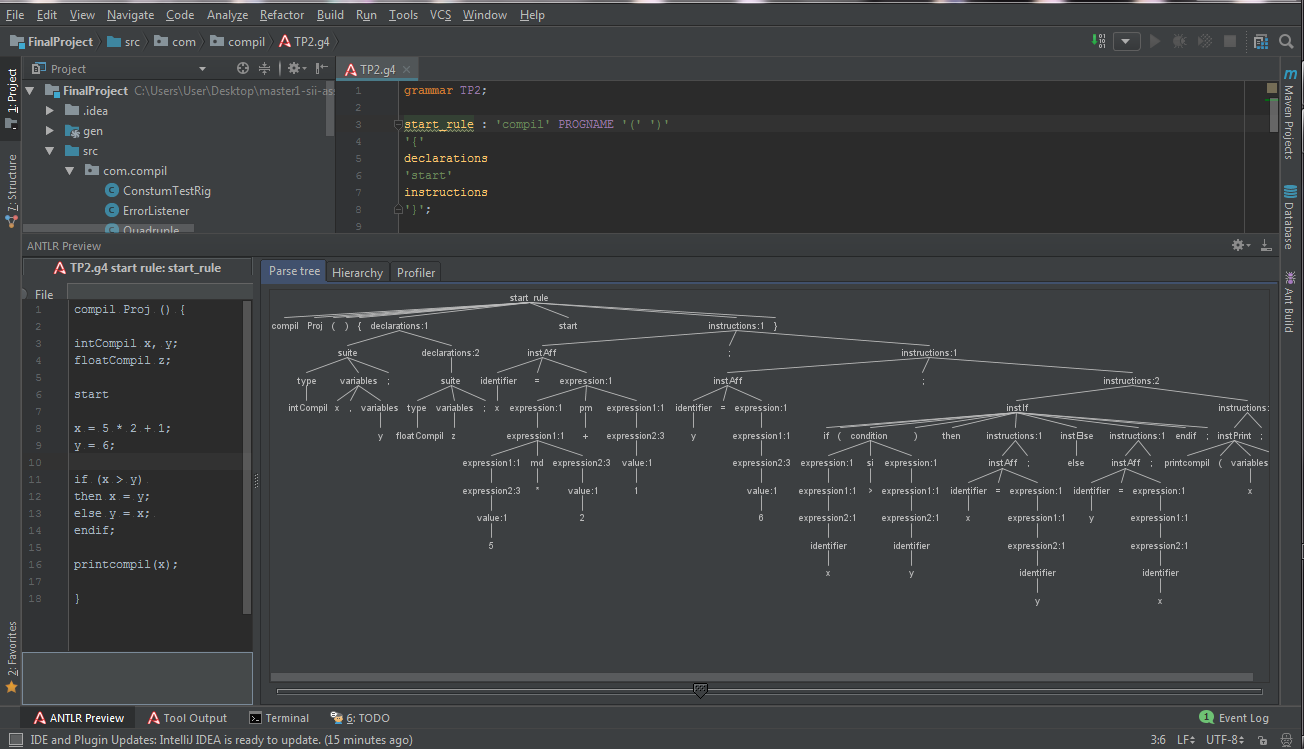
\includegraphics[width=1\textwidth]{IMG/TestRule2.png}
\texttt{ }\\
Et si un ou plusieurs conflits ont été détecté, l'arbre affichera l'emplacement du conflit.\\

\texttt{ }\\
-	Interface et organisation des codes\\
\texttt{ }\\
L'image ci-dessous montre comment les codes sont organisés dans notre projet:\\
- Dossier \textbf{gen:} qui contient les fichiers généré par ANTLR.\\
- Dossier \textbf{src:} qui contient les fichiers que nous avons crée pour les trois types d'analyse.\\
- Fichier \textbf{input.compil:} qui contient le code a tester, écrit dans le langage développé.\\
- Fichier \textbf{Assembly:} vide à la base, mais destiné à etre rempli suite à l'exécution du projet par le code objet correspondant au code testé.\\
\texttt{ }\\
%image Interface
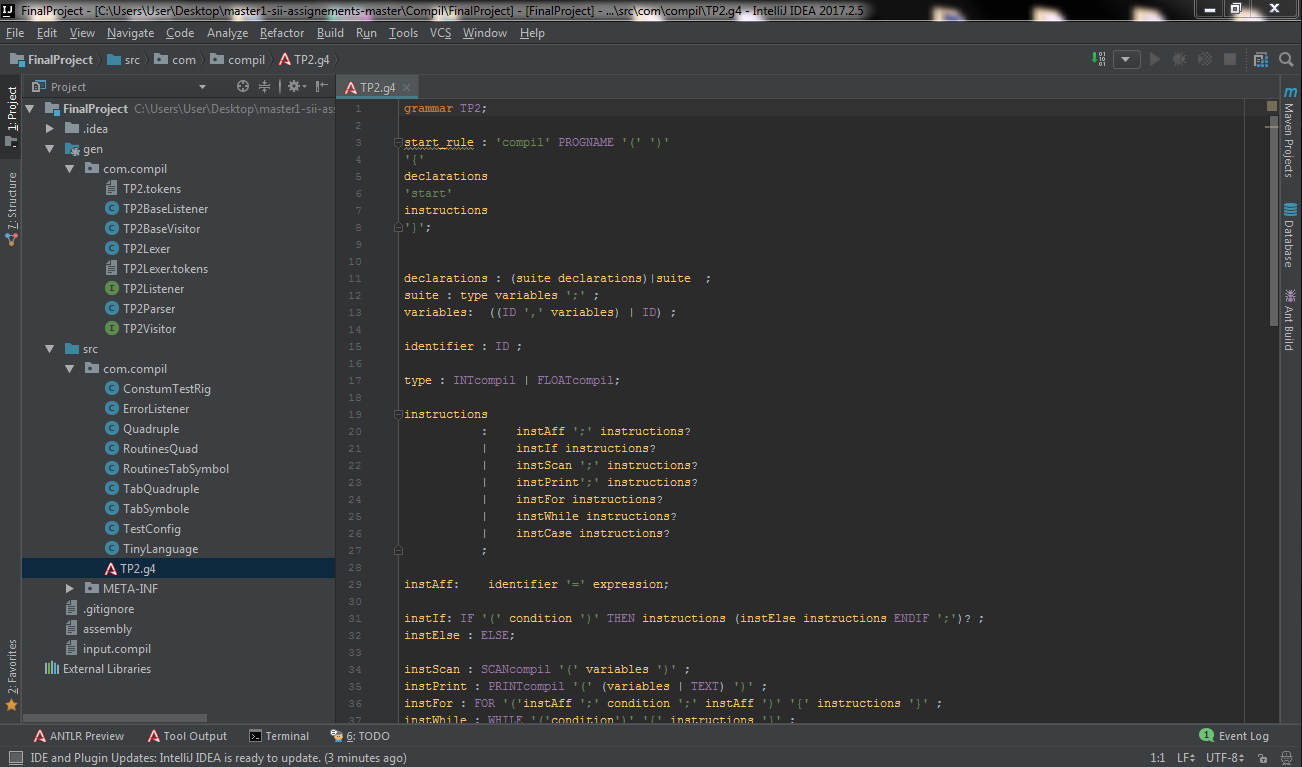
\includegraphics[width=1\textwidth]{IMG/Interface.png}


\texttt{ }\\
-	Création de la classe MyListner\\
\texttt{ }\\
Dans notre projet afin de mieux concevoir et gérer nos routine, nous avons opté pour deux classe héritant de BaseListner (c'est a dire nous avons deux (2) classe Mylistner).\\
1. Classe \textbf{RoutinesTabSymbol}: pour tout se qui est en relation avec la Table des Symboles et les routines sémantique.\\
2. Classe \textbf{RoutinesQuad}: pour la génération des Quadruplets et du code Objet.\\ 

\subsubsection{Génération du Code Intermédiaire}

Afin de générer nos quadruplets nous avons crée plusieurs classes, tel que :\\

\color{blue}
-	Quadruple :\\
\color{black} représentant la structure d'un quadruplet, c'est-à-dire les quatre (4) champs dont est composé un quadruplet (opération, opérande1, opérande2, temporaire) ;\\
 ainsi que les actions (méthodes) applicable sur ces derniers, nous citons : le constructeur, les getteurs et les setteurs.\\
 
\color{blue}
-	TabQuadruple :\\
\color{black} constitue la une table de quadruplet (LinkedList d'éléments de la classe Quadruple) en plus des opérations élémentaire dont :\\

Ajouter un quadruplet a la liste\\
Mise à jours d'un quadruplet (pour les branchement)\\
Récupérer un quadruplet d'après son indice dans la liste\\
Récupérer la taille de la liste\\
Affichage de la table des quadruplets entièrement\\ 

\color{blue}
-	RoutinesQuad :\\
\color{black} cette classe hérite du « BaseListener », elle contient principalement les méthodes de création de quadruplets selon l'événement rencontré (enter ou exit d'une règle de la partie syntaxique).\\
Faisant usage d'une LinkedList géré comme une pile afin d'empiler les opérandes des expressions arithmétiques pour gérer les priorités.\\


\color{red}
 Conclusion :\\
\color{black}
Ainsi lorsque nous serons en train de « parser » notre échantillon de code respectant la syntaxe de notre langage,\\
à chaque rencontre d'une règle  possédant un listner dans notre classe « RoutinesQuad »  le quadruplet correspondant sera construit puis inséré dans la table des routines instanciées à partir de la classe « TabQuadruple » ,\\
 puis nous pouvant les afficher ou/et les utiliser par la suite ;
Dans notre cas nous avons affiché la table des quadruplets puis utilisé cette table pour la génération du code Objet qui constitue la prochaine section.\\
\texttt{}\\

\subsubsection{Génération du Code Objet}

Nous avons fait quelques modifications sur la base du code obtenu lors de la phase précédente « génération des quadruplets », plus exactement sur les classes suivantes :\\

\color{blue}
-	TabQuadruple : \color{black} dans la quelle nous avons ajouter deux (2) méthodes :\\

o	La \textbf{première} permet de remplir une ArrayList « assembly » en bouclant sur tous les quadruplets de la table et de les traduire en langage assembleur avec la méthode « toAssembler » que nous avons développé dans la classe Quadruple.\\

\begin{sql}
    public ArrayList<String> toAssembly() {
        ArrayList<String> assembly = new ArrayList<>();
        int i =0;
        for (Quadruple q:quads){
            assembly.addAll(q.toAssembler(i));
            i++;
        }
        return assembly;
    }
\end{sql}

o	La \textbf{deuxième} permet d'écrire dans un fichier texte dont le chemin est donné en paramètre à partir de la ArrayList de code assembler obtenu grâce a la méthode juste au dessus.

\begin{sql}

    public void saveAssembly(String filename) throws IOException {
        Files.write(Paths.get(filename), toAssembly());
    }
\end{sql}

\color{blue}
-	Quadruple : \color{black} dans celle-ci nous avons ajouté des méthodes pour transformer un quadruplet en lignes de code assembleur sous forme d'une chaine de caractère ;
Tel que nous avons :\\

o	La \textbf{première} « toAssembler » permet principalement de vérifier le type d'opération que représente le quadruplet courant, tel que nous avons catégorisé cinq type d'opération sur les quadruplets, qui sont :\\
1/ opération arithmétique (+, -, *, / )\\
2/ affectation (=)\\
3/ branchement (BR, BGE, BLE)\\
4/ fin des quadruplets (Finale)\\
		Ainsi selon le type trouvé on fait appel à une méthode parmi :\\
		
o	La \textbf{deuxième}  « op » qui correspond au type (opération arithmétique) nous commençons par ajouter l'instruction assembleur :\\

\begin{sql}
assembly.add(mov(AX, op1));
\end{sql}

Qui nous donnera comme résultat une chaine de caractère (String) de la forme : « MOV AX, a » si op1 est une variable « a »\\

Puis selon l'opération en question une seconde instruction sera inséré, qui elle aussi aura la forme : « ADD AX, b » si op2 est une variable b et que l'opération est une addition.\\
Et enfin l'instruction qui met le résultat finale dans le temporaire, qui est comme suit : « MOV AX, Temp » ; avec Temps le temporaire.\\

//idém pour les autres instructions de soustraction, multiplication et division.\\

o	La \textbf{troisième} : « aff » permet de représenter l'affectation en assembleur, en deux instructions seulement, qui sont :\\
« MOV AX, op1 » puis «MOV Temp, AX »\\

o	La \textbf{quatrième} : «jump» quant a celle-ci elle vérifie d'abord s'il s'agit d'un jump conditionnelle ou inconditionnelle,\\

Dans le premier cas de figure nous insérant seulement une (1) instruction assembleur :\\
«  JMP etiq2 » ;\\
 avec etiq2 l'étiquette donnée comme deuxième opérande dans le quadruplet.\\

Dans le deuxième cas, quatre (4) instructions assembleurs sont générées : \\
«MOV AX, a» ;\\
 avec « a » la première opérande à comparer\\
«MOV BX, b» ;\\
 avec « b » la deuxième opérande à comparer\\
«CMP a, b»\\
«JLE etiq10» ou « JGE etiq10 » ;\\
 avec « etiq10 » l'étiquette à rejoindre en cas ou « a » est inférieur (resp supérieur) à « b »\\

o	En plus de vérifier a chaque instruction s'il s'agit d'une instruction vers la quelle il y a un JUMP (branchement) afin de la précéder par une étiquette.\\
Mais pour cela nous avons ajouté dans la classe « RoutinesQuad » un Vector contenant les numéros des quadruplets étiquettes (vers les quels il y a des branchements), et ce afin de les exploiter dans cette classe « Quadruple » tel que le numéro de quadruplet est passé en paramètre dans la première méthode cité « toAssembler».\\

\subsubsection{Classe Main}

Dans une classe du même nom que notre projet « TinyLanguage » nous avons notre main ;\\
Le main prends un tableau de string en paramètre d'entrée, ces paramètres peuvent être : -gui , -tree , -tokens , … mais un seul est obligatoire ! il s'agit du fichier texte contenant le code dans le langage développé a tester.\\

Pour tester nous avons d’abord instancié :\\
•	Un objet de la classe « TestConfig » lui donnant les argument du main en paramètre.\\
•	Une ArrayList errors pour accueillir les éventuelles erreurs que l'on rencontrera.\\
•	Un objet de la classe RoutinesTabSymbol qui génère la TS \\
•	Un objet de la classe RoutinesQuad qui génère la table des quadruplets\\
•	Une Liste ArrayList$<$TP2BaseListener$>$ routines afin d'y regrouper les routines de la TS ainsi que celles des Quadruplets comme suit : \\
        routines.add(routinesQuad);\\
        routines.add(routinesTabSymbol);\\

•	Un objet ErrorListener errorListener pour y recueillir les erreurs rencontrées en pour les afficher par la suite ou même procéder a un traitement par la suite.\\

•	Enfin on lance : ConstumTestRig.process(config, routines, errorListener) afin de générer le lexer et le parser \\

•	Puis nous nous retrouvons devant deux possibilités :\\
1.	Erreur rencontré : affichage de l'erreur rencontré.\\
2.	Aucune erreur : affichage de la TS, affichage des quadruplets, génération du code objet.\\


\subsubsection{Étapes de compilation du projet}

1. configurer la prise en charge du fichier "input.compil" contenant le code à tester:\\ 
Run $>$ Edit Configurations... $>$ Tab "Configuration" $>$ Program arguments\\
\texttt{ }\\
%image Config_Exe
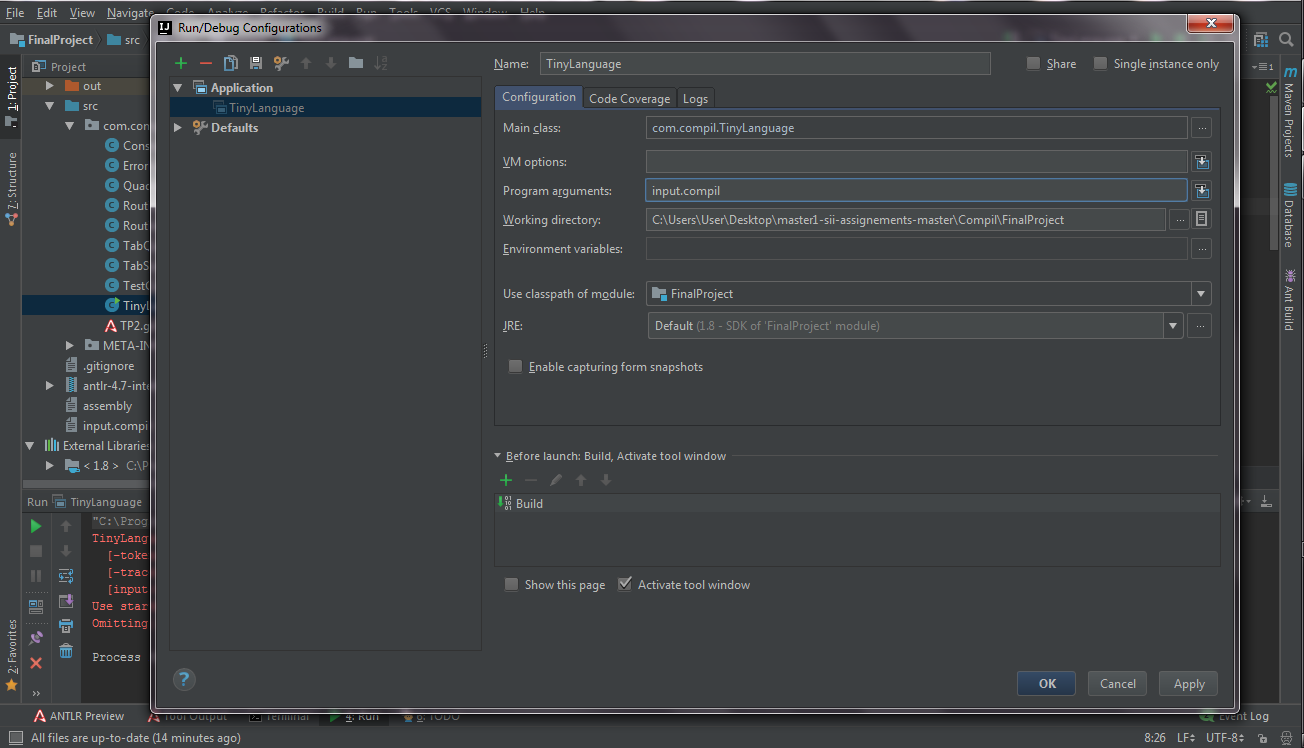
\includegraphics[width=1\textwidth]{IMG/Config_Exe.png}


\texttt{ }\\
2. lancer l'exécution:
Le lancement de l'exécution peut être réalisé a travers le bouton \texttt{run} de l'interface d'Intellij: \\

2.1 Affichage de la table des symboles Ainsi que des quadruplets généré.\\
\texttt{ }\\
%image Exe_TS_Quad
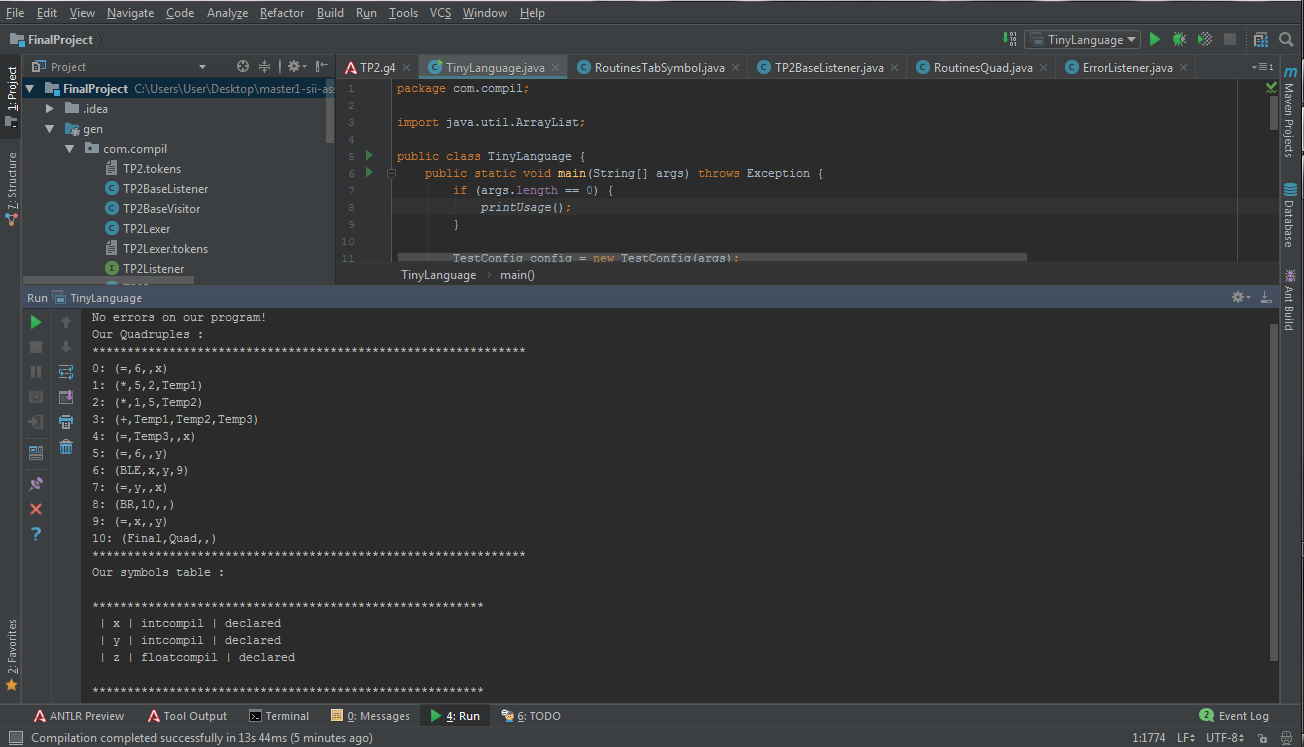
\includegraphics[width=1\textwidth]{IMG/Exe_TS_Quad.png}


\texttt{ }\\
2.2 Génération du code objet dans un fichier "Assembly"\\
\texttt{ }\\
%image Exe_Ojb
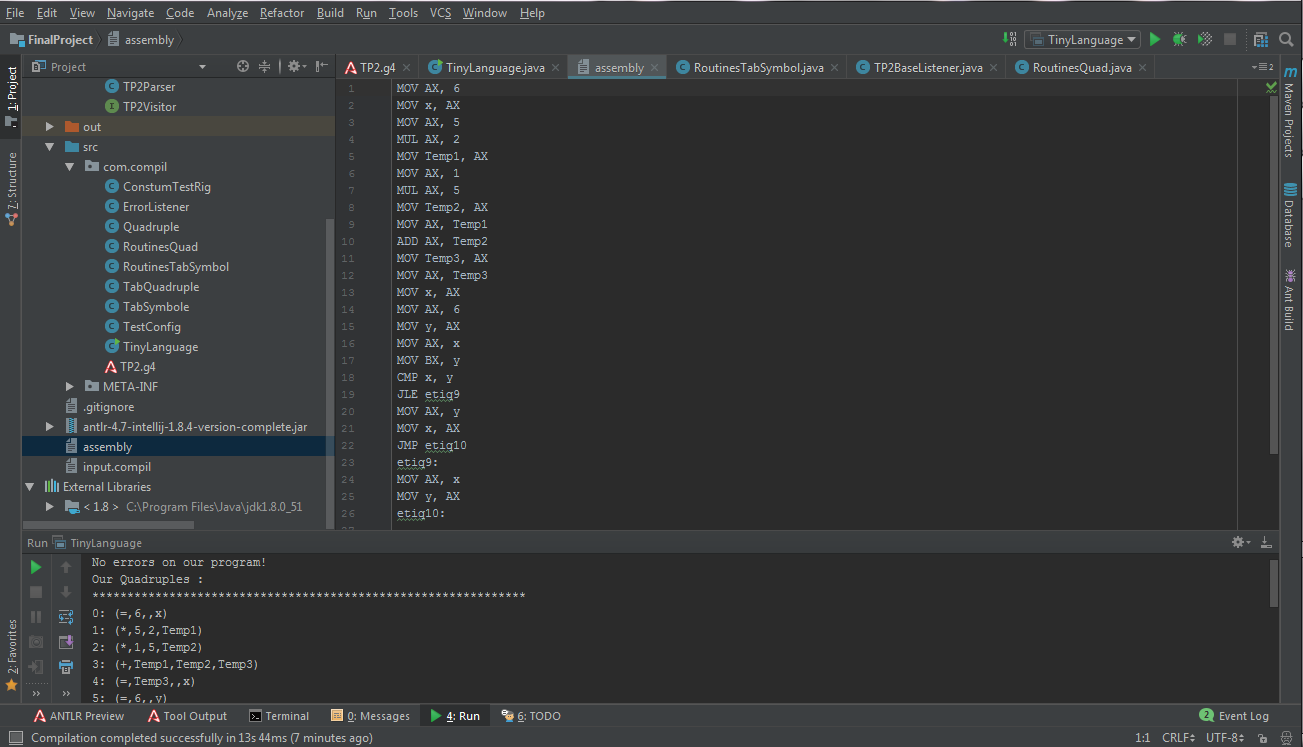
\includegraphics[width=1\textwidth]{IMG/Exe_Obj.png}


\texttt{ }\\
\subsection{Différence entre Flex/Bison et ANTLR}

La différence la plus significative entre YACC / Bison et ANTLR est le type de grammaire que ces outils peuvent traiter. 
YACC / Bison gère les grammaires LALR, ANTLR gère les grammaires LL.\\

YACC / Bison génère des analyseurs pilotés par table, ce qui signifie que la "logique de traitement" est contenue dans les données du programme analyseur,\\
 pas tellement dans le code de l'analyseur. L'avantage est que même un parseur pour un langage très complexe a une empreinte de code relativement faible.\\
 C'était plus important dans les années 1960 et 1970, lorsque le matériel était très limité. \\
 
 Les générateurs d'analyseurs pilotés par table remontent à cette époque et l'empreinte du petit code était une exigence principale à l'époque.\\

 
ANTLR génère des analyseurs de descente récursifs, ce qui signifie que la "logique de traitement" est contenue dans le code de l'analyseur,\\
 car chaque règle de production de la grammaire est représentée par une fonction dans le code de l'analyseur.\\ 
 
 L'avantage est qu'il est plus facile de comprendre ce que fait l'analyseur en lisant son code.\\
 En outre, les analyseurs de descente récursifs sont généralement plus rapides que les analyseurs pilotés par table.\\ 
 
 Cependant, pour les langues très complexes, l'empreinte du code sera plus grande. \\
 C'était un problème dans les années 1960 et 1970. 
 À l'époque, seuls des langages relativement petits comme Pascal par exemple étaient implémentés de cette façon en raison de limitations matérielles.\\

Les analyseurs syntaxiques générés par ANTLR sont généralement à proximité de 10.000 lignes de code et plus. \\
Les parseurs de descente récursifs manuscrits sont souvent dans le même ordre de grandeur. \\
Le compilateur Wirth's Oberon est peut-être le plus compact avec environ 4000 lignes de code incluant la génération de code, 
mais Oberon est un langage très compact avec seulement environ 40 règles de production.\\

Un grand avantage pour ANTLR est l'outil IDE graphique, appelé ANTLRworks. \\
C'est un laboratoire complet de grammaire et de langage. Il visualise vos règles de grammaire au fur et à mesure que vous les tapez et s'il trouve des conflits (s'il y en a), \\
il vous montrera graphiquement ce qu'est le conflit et ce qui le provoque. \\

Il peut même automatiquement refactoriser et résoudre des conflits tels que la récursivité à gauche. Une fois que vous avez une grammaire sans conflit, \\
vous pouvez laisser ANTLRworks analyser un fichier d'entrée de votre langage et construire une arborescence d'analyse 
et AST pour vous et afficher graphiquement l'arbre dans l'EDI. \\

C'est un très gros avantage car cela peut vous faire économiser beaucoup d'heures de travail: vous trouverez des erreurs conceptuelles dans votre langage avant de commencer à coder! nous n'avons pas trouvé un tel outil pour les grammaires LALR, il semble qu'il n'y en ait pas.\\

Il Peut produire des analyseurs syntaxiques dans différentes langages.\\

Et enfin Java n'est pas requis pour exécuter l'analyseur généré.\\



\section{Section Optionnelle.}
Lors de la réalisation de ce projet, nous avons pu apporter quelques améliorations à notre code, nous citons: \\

1. Ajout d'un \texttt{EndIf;} a la fin de l'instruction \texttt{IF} afin de délimiter la fin de la condition.\\

2. Création de la classe \texttt{CustomeTestRig}:\\
La classe \texttt{TestRig} par defaut produit énormément d'efforts afin de chercher, trouver et utiliser des information sur notre projet, tel que:\\
 le nom du projet, le nom de notre fichier .g4 , notre parser ainsi que notre listner, ... \\
 
afin de les instancier puis utiliser dans sa fonction \textbf{process} à la quelle nous faisons appel dans notre \textbf{Main}.\\ 

C'est pour cela que nous avons customiser notre classe \texttt{TestRig} lui donnant directement toutes ces informations nécessaire sur notre projet, et ainsi gagner en temps d'exécution.\\

3. Création de la classe \texttt{ErrorListner} : elle sert a récupérer les messages d'erreurs et de les afficher dans un format proche de celui des compilateur connu, en donnant le ligne et colonne ou se trouve l'erreur,\\
 mais aussi de sauvegarder ces erreurs en cas de besoin dans une utilisation ultérieure.\\


\end{document}
